\documentclass{standalone}
\usepackage{pgfplots}
\pgfplotsset{compat=1.17}

\begin{document}

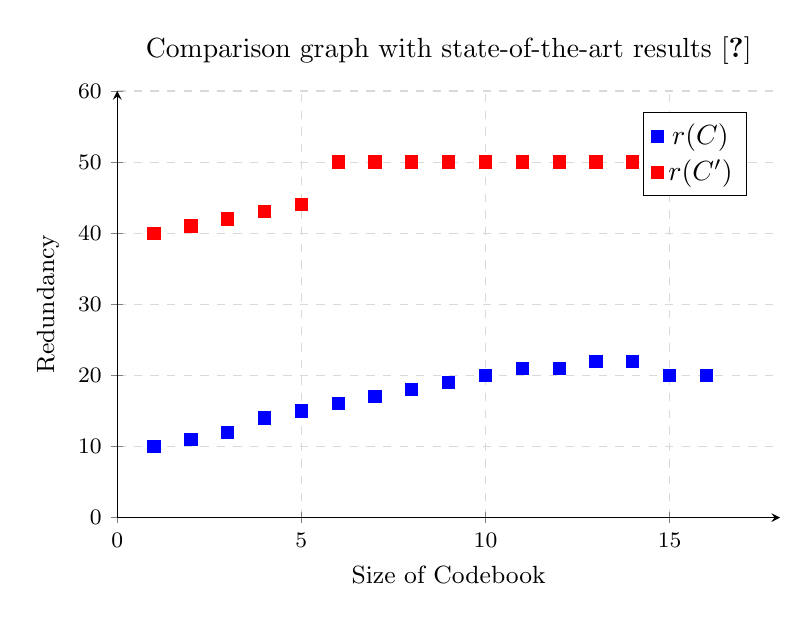
\begin{tikzpicture}
    \begin{axis}[
        title={Comparison graph with state-of-the-art results \cite{Smagloy_Welter_Wachter-Zeh_Yaakobi_2020}},
        xlabel={Size of Codebook},
        ylabel={Redundancy},
        xmin=0, xmax=18,
        ymin=0, ymax=60,
        xtick={0,5,10,15},
        ytick={0,10,...,60},
        legend pos=north west,
        grid=major,
        grid style={dashed, gray!30},
        width=10cm,
        height=7cm,
        axis lines=left,
        enlargelimits=false,
        legend style={at={(0.95,0.95)},anchor=north east},
        ticklabel style={font=\footnotesize},
        label style={font=\small},
        every axis plot/.append style={thick},
    ]

        % Plot for r(C)
        \addplot[
            only marks,
            mark options={mark size=2pt, fill=blue},
            mark=square*,
            color=blue,
            mark options={solid},
        ] coordinates {
            (1,10) (2,11) (3,12) (4,14) (5,15) (6,16) (7,17) (8,18) (9,19) (10,20) (11,21) (12,21) (13,22) (14,22) (15,20) (16,20)
        };
        \addlegendentry{$r(C)$};

        % Plot for r(C')
        \addplot[
            only marks,
            mark options={mark size=2pt, fill=red},
            mark=square*,
            color=red,
            mark options={solid},
        ] coordinates {
            (1,40) (2,41) (3,42) (4,43) (5,44) (6,50) (7,50) (8,50) (9,50) (10,50) (11,50) (12,50) (13,50) (14,50) (15,50) (16,50)
        };
        \addlegendentry{$r(C')$};

    \end{axis}
\end{tikzpicture}

\end{document}